The mathematical framework for probability involves set theory.

\subsection{Sample Spaces and Events}

\begin{example}[Sample Spaces]
  \begin{itemize}
    \item Toss a coin: $S=\{\text{Head},\text{Tail}\}$.
    \item Toss two coins: $S=\{(H,H),(H,T),(T,H),(T,T)\}$.
    \item Roll a die: $S=\{1,2,3,4,5,6\}$.
    \item Permute $1$--$6$: $S=\{123456,213456,312456,\ldots\}$.
  \end{itemize}
\end{example}

\begin{definition}{Outcomes and Events}{outcomes-events}
  An element of a sample space is an \textbf{outcome}.
  A subset of a sample space is an \textbf{event}.
\end{definition}

\begin{example}[Sum of Two Dice]
  \[
    E=\{\text{sum of two dice rolls is }7\}
    =\{(1,6),(2,5),\ldots,(6,1)\}\subseteq S,
  \]
  where $S$ is the sample space of two dice rolls.
\end{example}

\subsection{Probability}

Write $EF=E\cap F$ for intersection.

\begin{definition}{Probability}{probability}
  A probability on a sample space $S$ is a function $P$ defined on subsets of $S$ with properties:
  \begin{enumerate}
    \item $\forall E\subseteq S,\quad 0\le P(E)\le1$.
    \item $E,F\subseteq S$ and $EF=\varnothing$ imply
          \[
            P(E\cup F)=P(E)+P(F).
          \]
    \item $P(S)=1$.
  \end{enumerate}
\end{definition}

\begin{example}[Comparing Two Dice Rolls]
  \begin{align*}
    S & =\{(1,1),(1,2),\ldots,\text{all two-dice rolls}\},              \\
    E & =\{\text{outcome of first roll}>\text{outcome of second roll}\} \\
      & =\{(2,1),(3,1),(3,2),\ldots\}.
  \end{align*}
  By property (2) of Definition~\ref{def:probability},
  \[
    P(E)=P(\{(2,1)\})+P(\{(3,1)\})+P(\{(3,2)\})+\cdots.
  \]
\end{example}

\subsection{Some Properties}

\begin{theorem}{Properties of Probability}{probability-properties}
  \begin{enumerate}
    \item $P(\varnothing)=0$.
    \item $P(E)+P(E^c)=1$, where $E^c=S\setminus E$.
    \item $P(A\cup B)=P(A)+P(B)-P(AB)$.
  \end{enumerate}
\end{theorem}

\begin{proof}
  \begin{enumerate}
    \item Since $S\varnothing=\varnothing$ and $S\cup\varnothing=S$,
          \[
            P(\varnothing)+P(S)=P(S)\implies P(\varnothing)=0.
          \]
    \item Since $EE^c=\varnothing$ and $E\cup E^c=S$,
          \[
            P(E)+P(E^c)=P(S)=1.
          \]
    \item Since $A\cup B=A\cup(BA^c)$,
          \begin{center}
            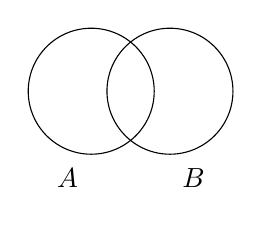
\begin{tikzpicture}
              \draw (0,0) circle (0.8);
              \draw (1,0) circle (0.8);
              \node at (-0.3,-1.1) {$A$};
              \node at (1.3,-1.1) {$B$};
            \end{tikzpicture}
          \end{center}
          \[
            P(A\cup B)=P(A\cup BA^c)=P(A)+P(BA^c).
          \]
          Also, $BA\cap BA^c=\varnothing$ and $BA\cup BA^c=B$, so
          \[
            P(B)=P(BA)+P(BA^c).
          \]
          Hence $P(A\cup B)=P(A)+P(B)-P(AB)$.\qedhere
  \end{enumerate}
\end{proof}

\begin{theorem}{Inclusion--Exclusion}{inclusion-exclusion}
  Generalizing property (3) of Theorem~\ref{thm:probability-properties},
  \begin{align*}
    P\left(\bigcup_{i=1}^n E_i\right)
     & =\sum_{i=1}^n P(E_i)-\sum_{1\le i<j\le n}P(E_iE_j) \\
     & \quad+\sum_{1\le i<j<k\le n}P(E_iE_jE_k)-\cdots    \\
     & \quad+(-1)^{n+1}P(E_1E_2\cdots E_n).
  \end{align*}
\end{theorem}

\subsection{Equally Likely Outcomes}

Let $\#S$ denote the number of elements in $S$. We usually have $\#S<\infty$.
Many times it is reasonable to consider all outcomes equally likely. Then
\[
  E\subseteq S\implies P(E)=\frac{\#E}{\#S}.
\]

\begin{example}[Poker: Flush]
  $E=\{\text{all cards in the same suit}\}$, and $S$ is the set of all possible five-card hands.
  \[
    \#S=\binom{52}{5},\qquad \#E=4\binom{13}{5}.
  \]
  Thus
  \[
    P(\text{flush})=\frac{4\binom{13}{5}}{\binom{52}{5}}
    =\frac{4\cdot13!\cdot47!}{8!\cdot52!}.
  \]
\end{example}

\begin{example}[Red and Blue Balls]
  Order $m$ red balls and $n$ blue balls in a row. How many different color arrangements are there?

  Label the balls $r_1,r_2,\ldots,r_m$ and $b_1,b_2,\ldots,b_n$.
  There are $(m+n)!$ ways to arrange them, and
  \[
    P(\text{a color arrangement})=\frac{m!\,n!}{(m+n)!}.
  \]
\end{example}
